\chapter{MiCS Implementation}
	... indledning ...

\section{Types in MiCS} % (fold)
\label{sec:types_in_mics}
	To help understand the core type validation and MiCS type mapping in general its beneficial to realise the different kind of types that are utilized in MiCS.

	\begin{figure}[H]
		\begin{center}
			\centerline{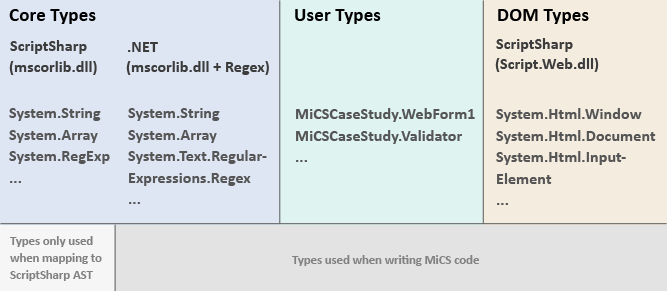
\includegraphics[width=16cm]{resources/images/TypesOverview.png}}
		\end{center}
		\caption{Illustrates the different types used by MiCS.}
		\label{typesOverview}
	\end{figure}

	Since one of the goals of MiCS is to be able to execute the same code on both client and server side (server client portability) its required that the .NET core types are used when writing MiCS code. This is in contrast to how Script\# works in its original manner where the Script\# core types (that reflect the equivalent JavaScript types) are used. This has some benefits but is also an obstacle that prevents server client portability.

	\subsection{Core Types} % (fold)
	\label{sub:core_types}
		To build the ScriptSharp AST correctly the ScriptSharp core types are required to be associated to the AST nodes. One reason why the ScriptSharp core types are required is that they define their equivalent script name (in the class attributes) that is used by the ScriptSharp script generator. An example is the System.Char (see figure \ref{char}) type which is converted to the JavaScript String type as no JavaScript Char type exists.

	\begin{figure}[H]
		\begin{center}
			\centerline{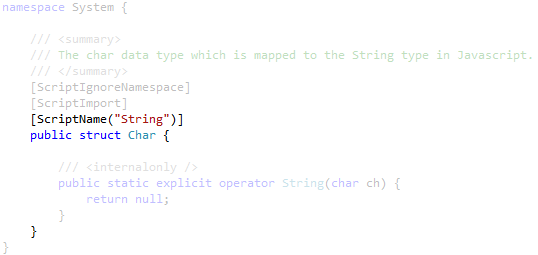
\includegraphics[width=13cm]{resources/images/Char.png}}
		\end{center}
		\caption{The core type System.Char defined in the Script\# mscorlib.dll.}
		\label{char}
	\end{figure}

	MiCS utilizes the regular .NET core types when a user is writing MiCS code but when generating the client side script the Script\# defined core types are used. This implies that some kind of mapping between the two kinds of core types are required. This mapping of core types is explained in section \ref{sub:type_mapping}.
	% subsection core_types (end)

	\subsection{User Types} % (fold)
	\label{sub:user_types}
		...
	% subsection user_types (end)

	\subsection{DOM Types} % (fold)
	\label{sub:dom_types}
		...
	% subsection dom_types (end)

% section types_in_mics (end)

\section{Validating Mixed and Client Side Code} % (fold)
\label{sec:syntax_tree_validation}
	% As we only support a fairly limited set of C\#’s built-in constructs and types, it is important to make sure that users only make use of those that we are able to map to Script\#. Should users utilise one of the constructs or types that we are not able to map, this should be pointed out with an understandable error message. It should not be left to the users to debug or understand a Roslyn or Script\# exception. Furthermore, it is important to make sure that users use their own code correctly. The remainder of this section will describe how a Validator class is used to achieve this.

	Before the Roslyn AST is mapped to Script\# it is necessary to verify that types and their members are used correcly. This is handled by the \texttt{Validator} class. If the developer only uses .NET types that we can map to Script\# and adhere to the Mixed Side Principle, the validation passes. The remainder of this section focus on how this validation is done.
	%Understanding “correct usage of .NET built-in types and members” is straightforward; it means that users are only allowed to use the types and members that can be mapped correctly to Script\#. How this is achieved is described later in this section. However, “correct usage of the types defined by the users themselves” requires some explanation. For this, the MixedSide Principle is introduced.

%To explain correct usage of types and their members, it is beneficial to divide them into two categories; types that are built into the .NET platform and types developers define themselves.



There are essentially three situations in which it is necessary to verify correct usage of types and members.

\begin{itemize}
	\item Object creation; when an instance of a type is created, it is necessary to check the type in question can be mapped.
	\item When members on type instances are accessed; it is then necessary to check first if the type can be mapped, then if the type has a member corresponding to the one being accessed.
	\item Invocation of methods on .NET core types; it is then necessary to check whether the invocation is done correctly, using the correct arguments and return type. Normally, the C\# compiler complains if an invocation is done using an incorrect signature, but as the interface between .NET core types and Script\# core types does not always match, it is important to make sure that the Script\# core type has a member with the corresponding arguments and return type. An invocation that is perfectly legal on .NET core types might be illegal on Script\# core types.
\end{itemize}

The \texttt{Validator} class extends Roslyn's \texttt{SyntaxWalker} class and it is thus able to traverse syntax nodes. The \texttt{Validator} takes a syntax tree that holds the source code to be validated, a string containing an attribute name (''MixedSide'' or ''ClientSide'') that decides what methods to validate, and a structure of types and members that can legally be used without violating the Mixed Side Principle. The \texttt{Validator} works by looking for classes in the syntax tree that contains methods annotated with the given attribute name and validates the body of these methods against the provided structure of allowed members.

The nature of the \texttt{Validator} requires the syntax tree to be validated twice. This is done by creating two instances of the Validator class, a \emph{MixedSide Validator} and a \emph{ClientSide Validator}, and validating them both. 
The MixedSide validator will do \emph{MixedSide validation} and the ClientSide validator will do \emph{ClientSide validation}:

\begin{itemize}
	\item \emph{MixedSide validation} requires validating all the \texttt{MixedSide} methods against a structure containing all \texttt{MixedSide} types and their members
	\item \emph{ClientSide validation} requires validating all the \texttt{ClientSide} methods against a structure containing all \texttt{ClientSide} types and members, \texttt{MixedSide} types and members and Script\# DOM types and members.
\end{itemize}


The Validation process is best explained by looking at an example. Consider a syntax tree holding the simple piece of code shown in figure \ref{fig:mixedSideValidationExample}. The methods of \texttt{ExampleClass} are subjects for MixedSide validation.

\begin{figure}[H]
	\begin{lstlisting}[language=CSharp,classoffset=1,morekeywords={ExampleClass,AnotherExampleClass,MixedSide}]
namespace ExampleNamespace
{
  public class ExampleClass
  {
  	[MixedSide]
  	public void ExampleMethod()
  	{
  		var a = new AnotherExampleClass();
  	}
  }
  
  public class AnotherExampleClass
  {
  	[MixedSide]
  	public void AnotherExampleMethod() { }
  }
}
	\end{lstlisting}
	\caption{Code subject to MixedSide validation}
	\label{fig:mixedSideValidationExample}
\end{figure}		

The MixedSide Validator traverses the syntax tree and discovers the \texttt{ExampleClass} class. It then finds all of the class' methods and checks if they have the \texttt{MixedSide} attribute. When a method annotated with the MixedSide attribute is found, the MixedSide Validator visits it straight away, as shown in Figure \ref{fig:ValidatorVisitClassDeclaration}. 

\begin{figure}[H]
	\begin{lstlisting}[language=CSharp,classoffset=1,morekeywords={ClassDeclarationSyntax,SyntaxKind,MethodDeclarationSyntax,List}]
/// <summary>
/// Visits the ClassDeclaration and determines wether its members should be validated
/// </summary>
public override void VisitClassDeclaration(ClassDeclarationSyntax @class)
{
  List<MethodDeclarationSyntax> methods = @class.DescendantNodes().Where(a => a.Kind == SyntaxKind.MethodDeclaration);
  bool visit = false;

  foreach (var method in methods)
  {
    visit = ((MethodDeclarationSyntax)method).HasAttribute(attributeName);

    if (visit)
      VisitMethodDeclaration((MethodDeclarationSyntax)method);
  }
}
	\end{lstlisting}
	\caption{Visiting a \texttt{ClassDeclarationSyntax} and deciding whether or not its methods should be validated}
	\label{fig:ValidatorVisitClassDeclaration}
\end{figure}


The first method visited is the \texttt{ExampleMethod()} method. The first statement of the method contains an object creation expression and the MixedSide Validator now needs to check if the object creation is legal. It is legal either if the created object is a supported core type, or if the created object is MixedSide type defined by the developer.



As the type exists in the allowed members structure (shown in figure \ref{fig:mixedSideValidationExample}) the object creation is legal and the traversal continues. If it had not existed in the allowed member structure (this could happen if it had been ClientSide), and had not been a supported core type, the MixedSide Principle would have been violated, and an exception of type \texttt{MixedSidePrincipleViolatedException} had been thrown.

The validation of a member access is done in a very similar way, only checking if the member exists in the allowed-members structure or in the core mapping as well.

As mentioned earlier, it is important to validate invocation on core types. This is done using the \texttt{VerifyCorrectUseOfSupportedCoreType} method on the \texttt{TypeManager}. This method first checks if the given invocation is done on a core type, and subsequently uses the Core Mapping Specification (as discussed in section \ref{sub:type_mapping}) to verify that we are able to map the invocation to ScriptSharp.
		



		% When an invocation is visited, the \texttt{TypeManager} is asked to 
		% TODO: Write about how invociations are validated: Only core types need to be validated (with arguments and return types), as user types will automatically be validated by the compiler.


% \begin{lstlisting}[language=CSharp,classoffset=1,morekeywords={TextBox,Panel,CheckBox, Button}]
% TextBox NameBox = new TextBox() { ID = "name", Text = "Name" };
% Panel CheckBoxGroup = new Panel();
% CheckBox SnailMailCheck = new CheckBox() { ID = "dmSnailmail", Text = "Snail Mail" };
% CheckBox EmailCheck = new CheckBox() { ID = "dmEmail", Text = "E-Mail" };
% TextBox AddressBox = new TextBox() { ID = "address", Text = "Address" };
% TextBox ZipcodeBox = new TextBox() { ID = "zipcode", Text = "Zip Code" };
% TextBox EmailBox = new TextBox() { ID = "email", Text = "E-mail" };
% TextBox PhoneBox = new TextBox() { ID = "phone", Text = "Phone" };
% Button SubmitButton = new Button() { Text = "Register" };
% \end{lstlisting}






	
	% subsection validating (end)
% section syntax_tree_validation (end)

\section{Mapping to ScriptSharp AST} % (fold)
\label{sec:mapping_to_scriptsharp_ast}
	When converting the validated Roslyn AST to the ScriptSharp AST we have made a logical division of the process. First the actual mapping from one Roslyn AST node to the equivalent ScriptSharp AST node. Secondly building the ScriptSharp AST from all the mapped nodes. The mapping is discussed in this section. 

	\subsection{Mapping to ScriptSharp Expressions, Statements and Symbols} % (fold)
	\label{sub:subsection_mapping_to_scriptsharp_expressions_statements_and_symbols}
		The mapping of Expressions, Statements and Symbols is implemented in three classes (ExpressionMapper.cs, StatementMapper.cs and SymbolMapper.cs). The three classes are logically divided (and named) after the type of ScriptSharp AST object they map to. 

		\begin{figure}[H]
			\begin{center}
				\centerline{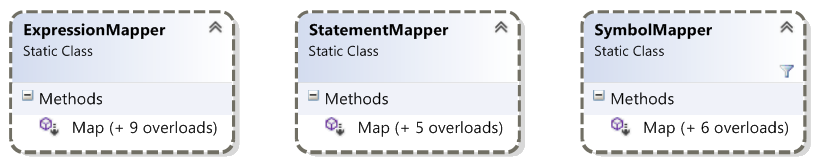
\includegraphics[width=14cm]{resources/images/MapperClasses.png}}
			\end{center}
			\caption{Classes that define extension methods for mapping Roslyn AST nodes to Script\# AST nodes.}
			\label{mapperClasses}
		\end{figure}

		The mapping of the AST nodes is somewhat straightforward as most of the mappings we have done the Roslyn AST maps one to one with the ScriptSharp AST. So a Roslyn return statement node maps to a ScriptSharp return statement etc. The three classes define Map(...) extension methods to the Roslyn objects they map from (see example figures \ref{returnStatementMap} and \ref{conditionaleExpressionMap}).

		\begin{figure}[H]
			\begin{center}
				\centerline{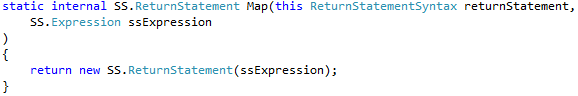
\includegraphics[width=14cm]{resources/images/ReturnStatementMap.png}}
			\end{center}
			\caption{Extension method that maps Roslyn return statement to Script\# return statement.}
			\label{returnStatementMap}
		\end{figure}

		\begin{figure}[H]
			\begin{center}
				\centerline{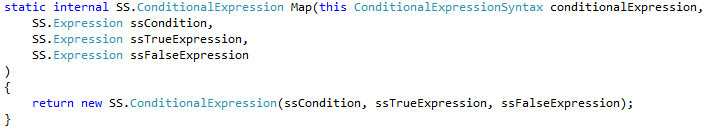
\includegraphics[width=14cm]{resources/images/ConditionalExpressionMap.png}}
			\end{center}
			\caption{Extension method that maps Roslyn conditional expression to Script\# conditional expression.}
			\label{conditionaleExpressionMap}
		\end{figure}
	% subsection subsection_mapping_to_scriptsharp_expressions_statements_and_symbols (end)

	\subsection{Type Mapping} % (fold)
	\label{sub:type_mapping}
		In contrast to using Script\# in the original manner (where the Script\# core types are used when writing code instead of the .NET core types) our project only uses the Script\# core types when mapping to the Script\# JavaScript AST. For this reason the Script\# core types are handled by its own type manager class (ScriptSharpTypeManager.cs). The Script\# core types’ source code are loaded into their own SemanticModel on the TypeManager class. From here the (Roslyn) types are retrieved before they are mapped to Script\# TypeSymbols needed when building the Script\# AST.

		Since the .NET core types are used when writing MiCS code and since these are mapped to the ScriptSharp core types a mapping specification is needed. To facilitate this mapping we have created some simple classes to hold the specification (MiCSCoreMapping.cs, MiCSCoreTypeMapping.cs and MiCSCoreMemberMapping.cs) which then can queried using LINQ. This mapping specification contains information on the core types that we currently support. So if a core type is not described in the specification then it is not supported. If the core type is found in the specification then the same pattern applies for its members. If a type member is not found then it is not supported. The mapping specification also holds information on a member’s return type, number of arguments and the arguments’ types.

		\begin{figure}[H]
			\begin{center}
				\centerline{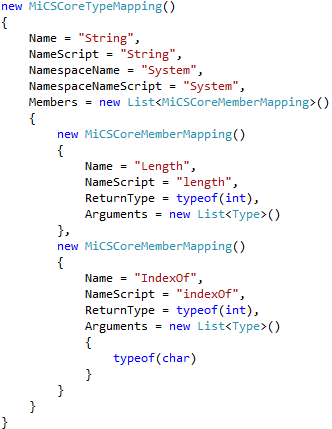
\includegraphics[width=8cm]{resources/images/InitiationOfTypeMapping.png}}
			\end{center}
			\caption{Instantiation example of a single core type (System.String) mapping specification.}
			\label{coreTypeMapping}
		\end{figure}

		An example of a core type mapping is the C\# System.String (see figure \ref{coreTypeMapping}) type which is mapped to the ScriptSharp defined System.String. We are only mapping two of the String type’s members. The field Length which is mapped to the ScriptSharp String type’s Length field (which is the equivalent of the JavaScript String object property length). The second member we map is the IndexOf(Char char) method that returns an int. There are other IndexOf methods that take multiple arguments or a single argument of a different type (than Char) but these are not mapped in our mapping specification.
	% subsection type_mapping (end)
% section mapping_to_scriptsharp_ast (end)

\section{Building the ScriptSharp AST} % (fold)
\label{sec:building_the_scriptsharp_ast}
	Building the Script\# AST consists of taking the mapped (Script\#) AST nodes and putting them together to form the Script\# AST. The builder classes utilize the Roslyn infrastructure by extending the SyntaxWalker class which makes them capable of traversing the Roslyn AST.
	\begin{figure}[H]
		\begin{center}
			\centerline{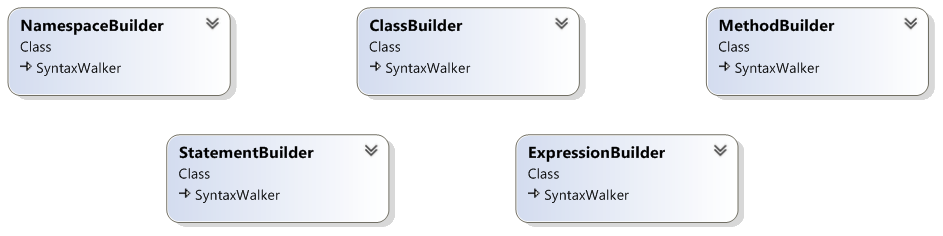
\includegraphics[width=16cm]{resources/images/BuilderClasses.png}}
		\end{center}
		\caption{Classes that built the Script\# AST by traversing the Roslyn AST and utilizing Map(...) extension methods.}
		\label{builderClasses}
	\end{figure}

	The NamespaceBuilder class is responsible for building all of its defined types. This is done by instantiating a ClassBuilder which in turn is responsible for building all of its member methods (which is done by instantiating a MethodBuilder). This implies that the building of the Script\# AST is done in a depth first manner. The NamespaceBuilder and ClassBuilder classes are somewhat trivial. 

	\begin{figure}[H]
		\begin{center}
			\centerline{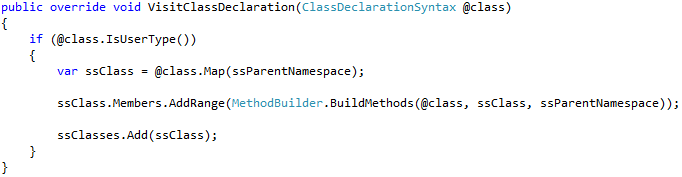
\includegraphics[width=16cm]{resources/images/VisitClassDeclaration.png}}
		\end{center}
		\caption{Empty Script\# class is created and then built by using a MethodBuilder to retrieve all its member methods. The ssClasses property on the builder holds all the classes that will be returned to the NamespaceBuilder who created this class builder.}
		\label{visitClassDeclaration}
	\end{figure}

	The ClassBuilder has an important feature that it ensures that only user defined types will be mapped to the Script\# AST (and generated as script types). DOM (or core) types doesn’t need to be defined in script as these obviously already exists in JavaScript.

	The MethodBuilder class is a little more complex as it needs to only build a method if its a MixedSide or ClientSide method. Furthermore it needs to handle a method’s return type, arguments and body statements. The StatementBuilder and ExpressionBuilder is however the most complex as building compound statements and expressions are more complicated. Before a compound statement or expression can be build all the child nodes and their associated types (if any) needs to be mapped.

	\begin{figure}[H]
		\begin{center}
			\centerline{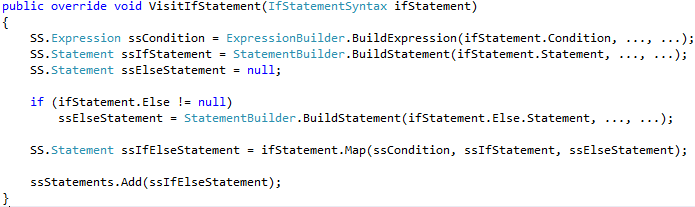
\includegraphics[width=16cm]{resources/images/VisitIfStatement.png}}
		\end{center}
		\caption{To built an IfStatement node its child nodes; condition, if-block and else-block (if any) has to be built first.}
		\label{visitIfStatement}
	\end{figure}

	When a builder class is done building the node(s) are returned to the parent builder class. Once all the namespaces has been built these constitute the Script\# AST which is then passed on in the overall workflow (to script generation).
% section building_the_scriptsharp_ast (end)

\section{Script Generation} % (fold)
\label{sec:script_generation}
	Script generation is done using the ScriptSharp infrastructure only. Specifically the TypeGenerator class located in the ScriptSharp.Generator namespace is utilized for this. The MiCSManager is responsible for instantiating the TypeGenerator and providing it with the ScriptSharp JavaScript AST type nodes (this happens in the MiCSManager.GenerateScriptText method). The ScriptSharp JavaScript AST consists only of the user defined script types.
% section script_generation (end)

\section{Integration with Web Forms} % (fold)
\label{sec:integration_with_web_forms}
	sdsadq qdqw qwd qwd qw 
% section integration_with_web_forms (end)
